% Social Event Recommendation Agent Project Proposal
\documentclass[10pt]{article}
\usepackage[a4paper,margin=1.35cm]{geometry}
\usepackage{booktabs}
\usepackage{array}
\usepackage{xcolor}
\usepackage{graphicx}
\usepackage{tabularx}

\definecolor{palBlue}{HTML}{4E79A7}
\definecolor{palOrange}{HTML}{F28E2B}
\definecolor{palGreen}{HTML}{59A14F}
\definecolor{palRed}{HTML}{E15759}
\definecolor{palPurple}{HTML}{B07AA1}
\definecolor{palGray}{HTML}{79706E}
\definecolor{palRule}{HTML}{D7D7D2}

\setlength{\parindent}{0pt}
\setlength{\parskip}{3pt}
\setlength{\tabcolsep}{4.5pt}
\renewcommand{\arraystretch}{1.06}
\newcolumntype{L}[1]{>{\raggedright\arraybackslash}p{#1}}
\newcolumntype{Z}{>{\raggedright\arraybackslash}X}

\newcommand{\sectiontitle}[1]{%
  \vspace{8pt}\noindent{\large\bfseries #1}\par\vspace{3pt}}
\newcommand{\subhead}[1]{\vspace{3pt}\noindent{\bfseries #1.}}
\newcommand{\smallcaps}[1]{\textsc{#1}}

\begin{document}

\begin{center}
{\LARGE\bfseries Social Event Recommendation Agent}\\[-1pt]
{\large Project Proposal}\\[-1pt]
Hochschule Bonn-Rhein-Sieg \textbar{} M.Sc. Autonomous Systems
\\Sunesh Praveen Raja Sundarasami
\end{center}
\vspace{-4pt}

\sectiontitle{1. Project Idea and Motivation}
The Social Event Recommendation Agent is a socially interactive recommendation agent for the Pepper robot in the \texttt{qiBullet} simulation environment. It detects a nearby user, initiates a short conversation, elicits preferences for social activities, and recommends suitable events. The project targets a realistic human--robot interaction problem: the user should not have to fill in a rigid form, but the robot must still make explainable, structured decisions.

The design combines three complementary components. First, a finite-state interaction manager controls the robot's visible behaviour and keeps the dialogue predictable. Second, a large language model (LLM) interprets natural answers and converts them into discrete evidence. Third, a Bayesian network performs transparent probabilistic reasoning over event categories. This keeps the final decision inspectable while still allowing natural language input.

\sectiontitle{2. Interaction Flow}
The robot follows a compact six-state cycle. In \smallcaps{Idle}, the camera waits for a stable face detection. In \smallcaps{Greeting}, Pepper waves and optionally addresses a recognized user by name. In \smallcaps{Conversation}, the robot asks for budget, group size, activity level, setting, time of day, and interest. In \smallcaps{Reasoning}, the LLM output is validated and passed to the Bayesian network. In \smallcaps{Recommendation}, the robot presents the top ranked events and explains why they match. In \smallcaps{Farewell}, it closes the interaction and returns to idle monitoring.

\begin{table}[h]
\small
\begin{tabularx}{\textwidth}{@{}L{2.7cm}ZZ@{}}
\toprule
\textbf{State} & \textbf{Robot action} & \textbf{Key transition} \\
\midrule
\smallcaps{Idle} & Passive camera monitoring & Face stable for several frames \\
\smallcaps{Greeting} & Wave, speech greeting, optional name & User remains present \\
\smallcaps{Conversation} & Preference questions with clarification & Required evidence complete \\
\smallcaps{Reasoning} & LLM parsing and Bayesian inference & Posterior distribution computed \\
\smallcaps{Recommendation} & Top events, explanation, open-palm gesture & User acknowledges / timeout \\
\smallcaps{Farewell} & Goodbye speech and wave & Return to \smallcaps{Idle} \\
\bottomrule
\end{tabularx}
\end{table}

\sectiontitle{3. Technical Architecture}
\subhead{Perception} A webcam detector based on OpenCV Haar cascades or MediaPipe FaceDetection triggers the first state transition. A five-frame smoothing window prevents flickering caused by short missed detections. Optional face recognition supports personalized greetings, but the core system always falls back to a generic greeting.

\subhead{Dialogue and LLM layer} The dialogue manager decides which preference question to ask next and checks whether the collected evidence is complete. The LLM is used only as an interface layer: it maps free-form answers such as ``something cheap outside with a few friends'' to discrete evidence values such as low budget, outdoor setting, and small group size. Ambiguous answers trigger short clarification questions.

\subhead{Recommendation engine} The Bayesian network is implemented with \texttt{pgmpy}. Evidence variables encode user preferences; latent variables summarize venue, social, and energy properties; the output variable stores the posterior over event types. Variable elimination returns the ranked recommendations.

\subhead{Behaviour layer} Speech is generated with \texttt{ALTextToSpeech}; gestures are played with \texttt{ALAnimationPlayer}. The gesture set includes greeting waves, attentive nods, thinking poses, open-palm presentation gestures, and farewell waves. Gestures run alongside speech so the interaction feels coordinated rather than sequential.

\sectiontitle{4. Bayesian Recommendation Model}
The model is deliberately small enough to be explainable. Six observed evidence nodes feed into three intermediate latent factors, which then determine the event recommendation distribution. The LLM never changes the graph structure or the conditional probability tables; it only supplies evidence values extracted from dialogue.

\begin{figure}[h]
\centering
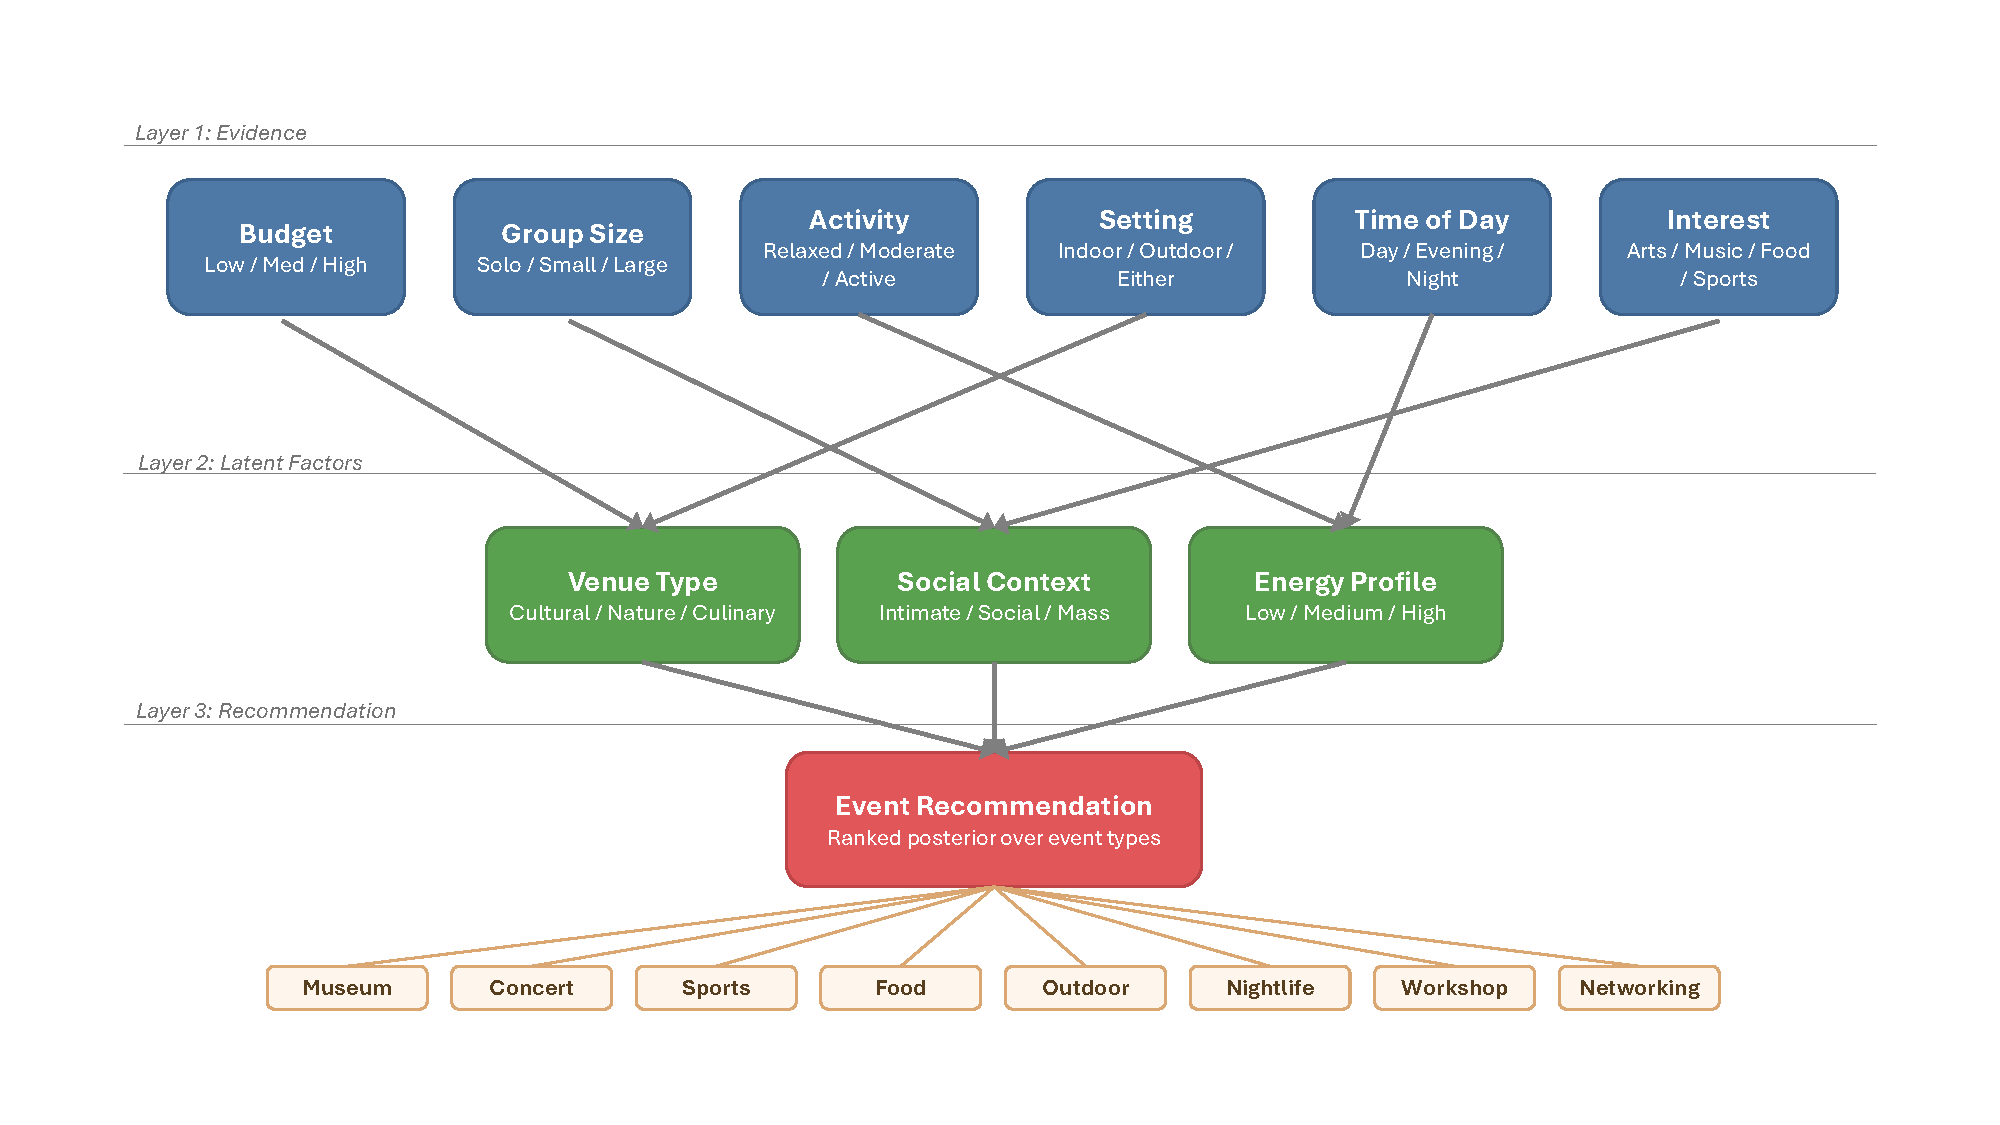
\includegraphics[width=\textwidth,trim=48 38 48 58,clip]{bayesian_flowchart.pdf}
\caption{Layered Bayesian recommendation graph. Evidence nodes are observed preferences, latent nodes summarize interpretable factors, and the output node ranks candidate events.}
\label{fig:bn}
\end{figure}

\begin{table}[h]
\small
\begin{tabularx}{\textwidth}{@{}L{2.2cm}ZZ@{}}
\toprule
\textbf{Layer} & \textbf{Variables} & \textbf{Role in inference} \\
\midrule
Evidence & Budget, GroupSize, ActivityLevel, Setting, TimeOfDay, Interest
& Directly elicited or LLM-parsed user preferences. \\
Latent & VenueType, SocialContext, EnergyProfile
& Compact abstractions that make the recommendation easier to explain. \\
Output & EventRec
& Posterior distribution over event categories; top three are presented. \\
\bottomrule
\end{tabularx}
\end{table}

\sectiontitle{5. Event Catalogue and CPT Basis}
\begin{table}[h]
\small
\begin{tabularx}{\textwidth}{@{}L{3.1cm}ZZZ@{}}
\toprule
\textbf{Event} & \textbf{VenueType} & \textbf{SocialContext} & \textbf{EnergyProfile} \\
\midrule
Museum / Gallery & Cultural & Intimate or Social & Low \\
Concert / Live Music & Entertainment & Social or Mass Event & Medium \\
Sporting Event & Entertainment & Mass Event & High \\
Food Festival & Culinary & Social or Mass Event & Low--Medium \\
Outdoor Adventure & Nature & Intimate & High \\
Night Club / Bar & Entertainment & Social & High \\
Workshop / Class & Cultural & Intimate & Medium \\
Networking Event & Cultural or Entertainment & Social & Medium \\
\bottomrule
\end{tabularx}
\end{table}

The event conditional probability table is therefore based on Layer 2, not directly on Layer 1. Evidence such as budget, setting, time, and interest first updates the latent factors VenueType, SocialContext, and EnergyProfile; the EventRec CPT then maps those latent factor combinations to event probabilities. For example, outdoor daytime answers increase the probability of the Nature and Low/High energy profiles, which then raises Outdoor Adventure or Food Festival depending on the inferred social context. This separation keeps the model explainable and lets it recover gracefully from incomplete or slightly inconsistent user answers.

\sectiontitle{6. Robustness and Safety}
\begin{table}[h]
\small
\begin{tabularx}{\textwidth}{@{}L{4.0cm}Z@{}}
\toprule
\textbf{Issue} & \textbf{Simple handling} \\
\midrule
Face is not detected reliably & Use a short smoothing window before starting the interaction. \\
User gives unclear answers & Ask one follow-up question or use a default value. \\
Some preferences are missing & Run the Bayesian network with the available evidence. \\
Recommendation seems weak & Present the top two or three events instead of only one. \\
Demo interruption & Return to the idle state and wait for the next user. \\
\bottomrule
\end{tabularx}
\end{table}

\sectiontitle{7. Evaluation Criteria}
The final demonstration will be evaluated with a small set of practical checks. The goal is not a full user study, but a working prototype that can detect a user, collect basic preferences, run the Bayesian model, and present a reasonable recommendation.

\begin{table}[h]
\small
\begin{tabularx}{\textwidth}{@{}L{4.0cm}Z@{}}
\toprule
\textbf{Check} & \textbf{Expected result} \\
\midrule
Face detection & Pepper starts the dialogue when a user is visible. \\
Dialogue & The robot asks the main preference questions once. \\
Parsing & User answers are converted into Bayesian evidence values. \\
Recommendation & The top events match the collected preferences. \\
Presentation & Pepper says the recommendation and performs a simple gesture. \\
\bottomrule
\end{tabularx}
\end{table}

\sectiontitle{8. Implementation Plan}
\begin{table}[h]
\small
\begin{tabularx}{\textwidth}{@{}L{1.4cm}Z@{}}
\toprule
\textbf{Week} & \textbf{Milestone} \\
\midrule
1 & Set up \texttt{qiBullet}; implement webcam detection and \smallcaps{Idle}$\rightarrow$\smallcaps{Greeting}. \\
2 & Build dialogue manager, LLM evidence parser, Bayesian variables, and initial CPTs. \\
3 & Connect inference, gesture library, recommendation presentation, and safety filters. \\
4 & Add optional speech input, face-recognition greeting, ranked explanations, and final demo tuning. \\
\bottomrule
\end{tabularx}
\end{table}

\sectiontitle{9. Conclusion}
The Social Event Recommendation Agent combines the flexibility of LLM-based language interpretation with the transparency of a Bayesian network. The user can speak naturally, while the system still reasons over explicit evidence and interpretable latent factors. The resulting robot interaction is compact, robust, explainable, and suitable for demonstrating socially aware event recommendation on Pepper.

\end{document}
